
\documentclass[journal,12pt,twocolumn]
{IEEEtran}
\usepackage[none]{hyphenat}
\usepackage{graphicx}
\usepackage{listings}
\usepackage[english]{babel}
\usepackage{graphicx}
\usepackage{caption} 
\usepackage{amsmath}
\usepackage{hyperref}
\usepackage{booktabs}
\usepackage{array}

\providecommand{\norm}[1]{\left\lVert#1\right\rVert}
\providecommand{\abs}[1]{\left\vert#1\right\vert}
\let\vec\mathbf
\newcommand{\myvec}[1]{\ensuremath{\begin{pmatrix}#1\end{pmatrix}}}
\newcommand{\mydet}[1]{\ensuremath{\begin{vmatrix}#1\end{vmatrix}}}
\providecommand{\brak}[1]{\ensuremath{\left(#1\right)}}




\title{\textbf{\\Assignment on conics}}
\author{Sireesha Abbavaram - FWC22060}
\begin{document}
\maketitle


\section{Question}\vspace{2mm}
\textbf{\textit{A hyperbola passes through the focus of the ellipse $x^2/25+y^2/16=1$.The transverse and conjugate axes of this hyperbola coincide with the major and minor axes of the given ellipse ,also the product of eccentricities of given ellipse and hyperbola is 1,then find focus of the hyperbola. 
}}
\vspace{5mm}

\section{Solution}

\begin{figure}[h!]
\centering
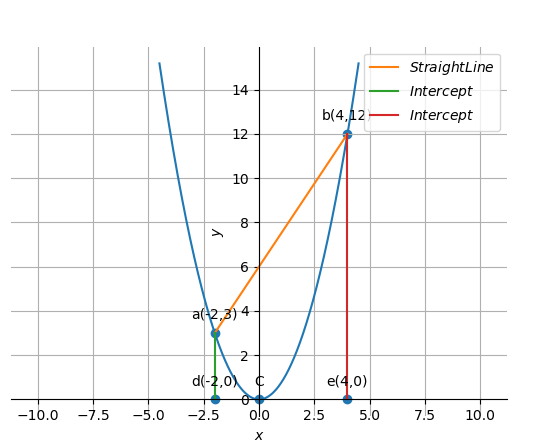
\includegraphics[scale=0.35]{conic.png}
\centering
\end{figure}

\begin{center}
The equation of a conic  is given by,
\end{center}
\begin{equation}
\vec{x}^{\top}\vec{V}\vec{x}+2\vec{u}^{\top}\vec{x}+f=0
\label{eq-1-}
\end{equation}

For the given equation of ellipse,


\begin{equation}
\vec{V} = \begin{pmatrix} 
	16 & 0 \\
	0 & 25 \\
	\end{pmatrix}, \hspace{4mm} \vec{u} = \myvec{0 \\ 0} \hspace{2mm} \& \hspace{2mm} f = -400
\label{eq-2-}
\end{equation}
The eigenvalue decomposition of a symmetric matrix $\vec{V}$ is given by
\begin{equation}
\vec{P}^{\top}\vec{V}\vec{P} = \vec{D} \hspace{1cm} 
\vec{P} = \myvec{\vec{P_1} & \vec{P_2}}
\label{eq-3-}
\end{equation}

\begin{equation}
\vec{D} = \begin{pmatrix} 
	\lambda_1 & 0 \\
	0 & \lambda_2 \\
	\end{pmatrix} 
\label{eq-4-}
\end{equation}
On solving $\eqref{eq-3-}$ with $\vec{P_1} = \myvec{1 \\ 0} \hspace{2mm} \& \hspace{2mm} \vec{P_2} = \myvec{0 \\ 1}$, we get
\begin{equation}
\vec{D} = \begin{pmatrix} 
	16 & 0 \\
	0 & 25 \\
	\end{pmatrix}
\label{eq-5-}
\end{equation}

\begin{equation}
\lambda_1 = 16 \hspace{2mm} and \hspace{2mm} \lambda_2 = 25
\label{eq-6-}
\end{equation}

\begin{equation}
eccentricity, \hspace{3mm} e = \sqrt{1-\frac{\lambda_1}{\lambda_2}}
\label{eq-7-}
\end{equation}
from $\eqref{eq-6-}$,
\begin{equation}
e1=3/5
\label{eq-8-}
\end{equation}
\begin{center}
Given that e1*e2=1
\end{center}
\begin{center}
so,eccentricity of hyperbola is e2=5/3
\end{center}
\begin{center}
Normal vector of diretrix $\vec{n}$ is given by
\end{center}
\begin{equation}
\vec{n} = \sqrt{\lambda_2}\vec{P_1}
\label{eq-9-}
\end{equation}
\begin{center}
This gives,
\end{center}
\begin{equation}
\vec{n} = \myvec{5 \\ 0}
\label{eq-10-}
\end{equation}
For e $\neq$ 1, we have
\begin{equation}
c = \frac{e\vec{u}^{\top} \vec{n}\pm \sqrt{e^2\brak{\vec{u}^{\top}\vec{n}}^2 - \lambda_2 \brak{e^2-1}\brak{\norm{\vec{u}}^2-\lambda_2 f }}}{\lambda_2 e \brak{e^2-1}}
\label{eq-11-}
\end{equation}
On solving we get,
\begin{equation}
c = \pm 41.67
\label{eq-12-}
\end{equation}
\begin{center}
Focii of a conic is given by the equation,
\end{center}
\begin{equation}
\vec{F} = \frac{ce^2\vec{n}-\vec{u}}{\lambda_2}
\label{eq-13-}
\end{equation}
Yelding,
\begin{equation}
\vec{F} = \pm 3
\label{eq-14-}
\end{equation}
Therefore, focii of the ellipse are,
\begin{equation}
\vec{F_1} = \myvec{-3 \\ 0} \hspace{2mm} \& \hspace{2mm} \vec{F_2} = \myvec{3 \\ 0}
\label{eq-15-}
\end{equation}
\begin{center}
From equation 7 we can write ,for hyperbola
\end {center}
\begin{center}
$\lambda_1/\lambda_2=1-e_2^2$
\end{center}
\begin{center}
so,$\lambda_1=-16$ and $\lambda_2=9$
\end{center}
\begin{center}
$\vec{P}^{\top}\vec{V}\vec{P} = \vec{D}=$ $\begin{pmatrix} 
	-16 & 0 \\
	0 & 9 \\
	\end{pmatrix} \hspace{1cm}$
\end{center}
\begin{center}
by soving we get
$\vec{V}=$ $\begin{pmatrix} 
	-16 & 0 \\
	0 & 9 \\
	\end{pmatrix} $ and
\end{center}
\begin{center}
$\vec{u} = \myvec{0 \\ 0}$
\end{center} 
\begin{center}
Since hyperbola is passing through $\vec{F_1}$
\end{center}
\begin{equation}
\vec{F_1}^{\top}\vec{V_1}\vec{F_1}+2\vec{u_1}^{\top}\vec{F_1}+f_1=0 
\label{eq-18-}
\end{equation} \vspace{1mm}
\begin{center}
by substituting above,we get
\end{center}
\begin{gather*}
\implies f_1 = 144
\end{gather*}

Hence, Equation of the hyperbola is given as,
\begin{equation}
-16x^2+9y^2+144=0
\label{eq-20-}
\end{equation}
\begin{center}
from $\eqref{eq-3-}$
\end{center}
\begin{equation}
\vec{n1} = \myvec{3 \\ 0}
\end{equation}
\begin{center}
from $\eqref{eq-11-}$
\end{center}
\begin{equation}
c1 = \pm 5.4
\label{eq-12-}
\end{equation}

\begin{center}
Focii of the hyperbola is given by the equation,
\end{center}
\begin{equation}
\vec{F} = \frac{ce^2\vec{n}-\vec{u}}{\lambda_2}
\end{equation}
Yelding,
\begin{equation}
\vec{F} = \pm 5
\end{equation}
Therefore, focii of the hyperbola are,
\begin{equation}
\vec{F_1} = \myvec{-5 \\ 0} \hspace{2mm} \& \hspace{2mm} \vec{F_2} = \myvec{5 \\ 0}
\end{equation}

\end{document}
